\documentclass[12pt]{article}
\usepackage{amsmath, amssymb, amsthm, tikz, pgfplots}
\usepackage{geometry, enumitem, mdframed, xcolor}
\geometry{margin=1in}

% Custom environments
\newtheorem{definition}{Definition}
\newtheorem{theorem}{Theorem}
\newtheorem{method}{Method}
\newtheorem{example}{Example}
\newmdenv[linecolor=blue,linewidth=2pt]{keypoint}
\newmdenv[linecolor=red,linewidth=2pt]{warning}
\newmdenv[linecolor=green,linewidth=2pt]{insight}

\title{ODE Lesson 10: Qualitative Analysis Without Solving}
\author{ODE 1 - Prof. Adi Ditkowski}
\date{}

\begin{document}
\maketitle

\section{Phase Line Analysis}

\begin{definition}[Phase Line]
For an autonomous ODE $\frac{dy}{dx} = f(y)$, the \textbf{phase line} is a one-dimensional representation showing equilibria and flow direction along the $y$-axis.
\end{definition}

\begin{method}[Constructing Phase Lines]
\begin{enumerate}
    \item Find equilibria: solve $f(y) = 0$
    \item Determine sign of $f(y)$ between equilibria
    \item Draw arrows: up if $f(y) > 0$, down if $f(y) < 0$
    \item Classify stability based on arrow directions
\end{enumerate}
\end{method}

\section{Stability Analysis}

\begin{theorem}[Linear Stability Test]
For $\frac{dy}{dx} = f(y)$ with equilibrium $y^*$:
\begin{itemize}
    \item If $f'(y^*) < 0$: asymptotically stable
    \item If $f'(y^*) > 0$: unstable
    \item If $f'(y^*) = 0$: test inconclusive (need higher derivatives)
\end{itemize}
\end{theorem}

\begin{example}[Logistic Equation]
For $\frac{dy}{dx} = ry(1 - y/K)$ with $r, K > 0$:
\begin{itemize}
    \item Equilibria: $y = 0$ and $y = K$
    \item $f'(y) = r(1 - 2y/K)$
    \item At $y = 0$: $f'(0) = r > 0$ (unstable)
    \item At $y = K$: $f'(K) = -r < 0$ (stable)
\end{itemize}
\end{example}

\section{Comparison Theorems}

\begin{theorem}[Basic Comparison Principle]
If $y_1(x)$ and $y_2(x)$ are solutions to $\frac{dy}{dx} = f(x,y)$ where $f$ satisfies uniqueness conditions, and $y_1(x_0) < y_2(x_0)$, then $y_1(x) < y_2(x)$ for all $x$ in the interval of existence.
\end{theorem}

\begin{keypoint}
Solutions cannot cross! This provides powerful bounds on solution behavior.
\end{keypoint}

\section{Monotonicity and Concavity}

\begin{method}[Analyzing Solution Shape]
For $\frac{dy}{dx} = f(x,y)$:
\begin{enumerate}
    \item \textbf{Monotonicity}: Sign of $f(x,y)$ determines if $y$ increases or decreases
    \item \textbf{Concavity}: Compute $\frac{d^2y}{dx^2} = \frac{\partial f}{\partial x} + \frac{\partial f}{\partial y} \cdot f$
    \item Positive second derivative $\Rightarrow$ concave up
    \item Negative second derivative $\Rightarrow$ concave down
\end{enumerate}
\end{method}

\section{Energy Methods and First Integrals}

\begin{definition}[First Integral]
A function $H(x,y)$ is a \textbf{first integral} of $\frac{dy}{dx} = f(x,y)$ if $H$ is constant along solution curves.
\end{definition}

\begin{theorem}[Exactness Criterion]
The ODE $M(x,y)dx + N(x,y)dy = 0$ is exact if $\frac{\partial M}{\partial y} = \frac{\partial N}{\partial x}$. When exact, solutions are level curves of $H(x,y)$ where $\frac{\partial H}{\partial x} = M$ and $\frac{\partial H}{\partial y} = N$.
\end{theorem}

\begin{insight}
Energy methods reveal hidden conservation laws and geometric structure!
\end{insight}

\section{Asymptotic Behavior}

\begin{method}[Determining Long-term Behavior]
\begin{enumerate}
    \item Identify all equilibria
    \item Analyze stability of each equilibrium
    \item Look for invariant regions (where solutions cannot escape)
    \item Apply comparison theorems for bounds
    \item Check for periodic orbits (closed trajectories)
\end{enumerate}
\end{method}

\section{Phase Line Examples}

\begin{example}[Phase Line for $y' = y(1-y)$]
\begin{center}
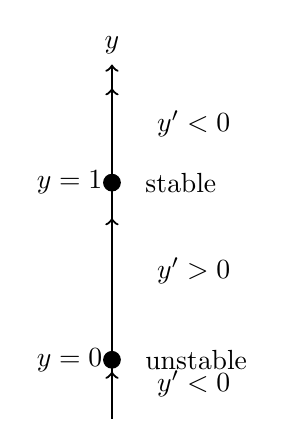
\begin{tikzpicture}[scale=1.5]
% Draw y-axis
\draw[thick,->] (0,-0.5) -- (0,2.5) node[above] {$y$};

% Mark equilibria
\filldraw (0,0) circle (2pt) node[left] {$y=0$};
\filldraw (0,1.5) circle (2pt) node[left] {$y=1$};

% Draw arrows
\draw[thick,->] (0,-0.3) -- (0,-0.1);
\draw[thick,->] (0,0.3) -- (0,1.2);
\draw[thick,->] (0,1.8) -- (0,2.3);

% Labels
\node[right] at (0.2,0) {unstable};
\node[right] at (0.2,1.5) {stable};
\node[right] at (0.3,-0.2) {$y' < 0$};
\node[right] at (0.3,0.75) {$y' > 0$};
\node[right] at (0.3,2.0) {$y' < 0$};
\end{tikzpicture}
\end{center}
\end{example}

\section{Periodic Solutions}

\begin{theorem}[Conditions for Periodicity]
\begin{itemize}
    \item Autonomous 1D equations cannot have periodic solutions
    \item For 2D systems, look for:
    \begin{itemize}
        \item Centers in linear analysis
        \item Conserved quantities (Hamiltonian systems)
        \item Application of Poincaré-Bendixson theorem
    \end{itemize}
\end{itemize}
\end{theorem}

\section{Exam Strategy}

\begin{warning}
Prof. Ditkowski's favorite qualitative analysis questions:
\begin{enumerate}
    \item Sketch phase line and determine all asymptotic behaviors
    \item Prove solution boundedness without solving
    \item Use comparison to relate unknown solutions to known ones
    \item Find conserved quantities for given ODEs
    \item Determine existence/non-existence of periodic solutions
\end{enumerate}
\end{warning}

\section{Memory Aids}

\begin{center}
\textbf{QUALITATIVE Analysis Steps:}\\
\textbf{Q}uick equilibrium check\\
\textbf{U}se stability tests\\
\textbf{A}nalyze monotonicity\\
\textbf{L}ook for conservation\\
\textbf{I}dentify invariant regions\\
\textbf{T}rack asymptotic behavior\\
\textbf{A}pply comparison theorems\\
\textbf{T}est for periodicity\\
\textbf{I}nterpret physically\\
\textbf{V}erify with phase line\\
\textbf{E}xamine concavity
\end{center}

\end{document}